\part{L'Intelligence Artificelle remplace l'humain pour les tâches répétitives}
\chapter{L'Intelligence Artificelle aujourd'hui}
L'intelligence Artificelle est un domaine faisant partie
des sciences cognitives dont l'objectif est de mettre au
point des techniques et des technologies permettant aux
machines de simuler l'intelligence humaine ou animale.
Nous pouvons réparatir les Intelligences Artificielles selon deux catégories distinctes.

\section{Intelligence Artificielle Faible}
Les IAs de cette catégorie cherchent à reproduire un comportement
répondant spécifiquement à un problème donné (ou une situation donnée)
le plus fidèlement possible.\newline

Pour s'approcher de ce comportement, l'IA de cette catégorie
va se baser sur l'apprentissage du comportement cible
mais n'en n'imite pas le fonctionnement ce qui fait que
ce type d'IA ne fait que simuler de l'intelligence.
Ce type d'IA ne prends pas en compte les problématiques et facteurs externes
qui influencent la décision de l'action à prendre. \newline

Aujourd'hui il n'existe que des intelligences artificelles faibles qui peuvent
être séparées en plusieurs technique et sous-domaines: \newline

\begin{figure}[H]
    \centering
    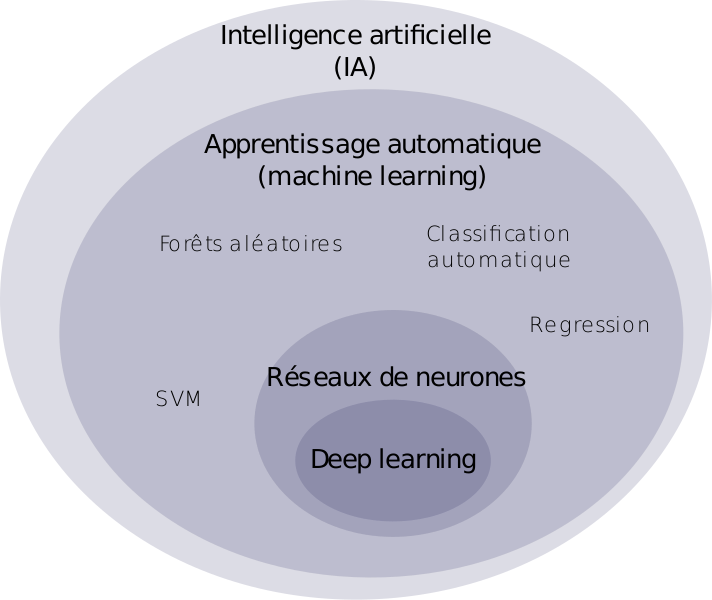
\includegraphics[width=0.7\textwidth]{Images/aitype}
    \caption{Les différents domaines de l'Intelligence Artificielle}
	\label{fig:DiffDomaineIA}
\end{figure}
\newpage

\subsection{Shallow Learning}
Le Machine Learning est un ensemble de techniques qui permettent à un ordinateur
d'agir et d'apprendre comme un humain tout en s'améliorant au fur et
à mesure et ce de manière autonome. \newline

Le fonctionnement du machine learning se découpe en plusieurs parties,
tout d'abord il faut définir des features, c'est-à-dire des
propriétés mesurables individuellement, cette partie est difficile et cruciale
car elle va déterminer l'efficacité de l'algorithme de machine learning. \newline

Différents algorithmes vont ensuite servir à extraire les features de données
brut en entrée avant de les envoyer à l'algorithme de machine learning, par exemple
la reconnaissance de bords ou de forme geométriques extrait les features d'une
image dans une IA de reconnaissance d'image. \newline

Enfin l'algorithme de machine learning va passer au travers de 3 ensembles de données:
\begin{itemize}
    \item un ensemble d'entraînement va permettre d'entraîner l'algorithme de manière
     supervisé, ce ensemble utilise des vecteurs d'entrée et leur sortie attendue.
    \item un ensemble de validation qui va verifier le modèle crée à partir de l'ensemble
    d'entraînement.
    \item un ensemble de test qui permet de tester la version finale de l'algorithme.
    \newline
\end{itemize}

Le machine learning utilise les "réseaux de neurones", qui ont fait leurs premières
apparition à partir de 1980, il s'agit de structures algorithmiques imitant
le comportement des neurones dans le cerveau humain:


\begin{figure}[H]
    \centering
    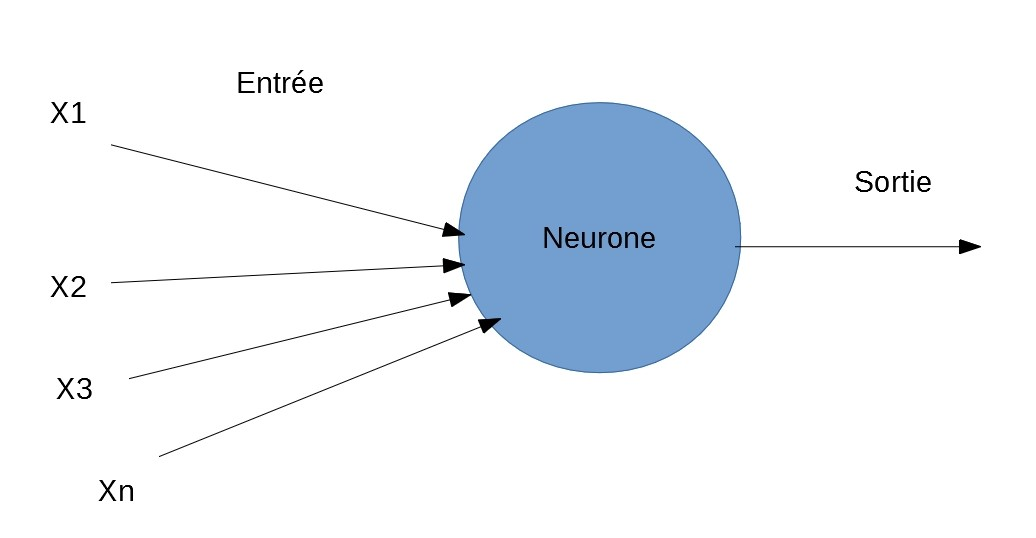
\includegraphics[width=0.6\textwidth]{Images/neuroneartificiel}
    \caption{Neurone Biologique et Neurone Artificel}
	\label{fig:NN2Layers}
\end{figure}

Un neurone artificiel comme son nom l'indique imite la topologie d'un neurone biologique,
ses entrées sont comparables aux dendrites d'un neurone tandis que sa
sortie est l'équivalent de l'axone. \newline

Les neurones sont répartis sur différentes couches: couche d'entrée, couche(s) cachée(s)
et couche de sortie. Dans le cas du "shallow learning" (apprentissage superficiel,
en opposition à l'apprentissage profond : "Deep Learning"), le réseaux de neurones
n'est composé que d'une seule couche cachée, c'est-à-dire une seule couche entre
la couche d'entrée et la couche de sortie:

\begin{figure}[H]
    \centering
    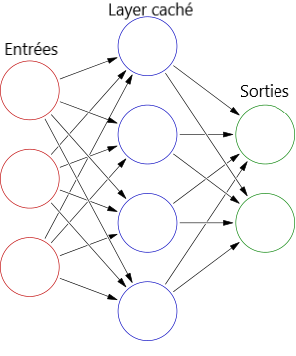
\includegraphics[width=0.4\textwidth]{Images/shallownnoverview}
    \caption{Réseau de neurones avec 2 couches cachées}
	\label{fig:NN2Layers}
\end{figure}

Ce type de réseaux de neurones est entrainé de manière supervisée.
L'IA va apprendre en utilisant des exemples qui auront été décrits
et expliqués (précision sur le dégré de validité) au préalable.

Mais dès lors qu'il y a plus d'une couche cachée,
il n'est plus possible de l'entrainer ainsi.
L'alternative qui répond à ce problème est l'apprentissage profond ou
Deep Learning qui utilise des réseaux de neurones avec de multiples couches
cachées.


\subsection{Deep Learning}
Le Deep Learning est une sous-catégorie du machine learning qui s'est démocratisé
qu'à partir de 2010 et est une évolution des anciennes techniques de Machine Learning.
La différence majeure entre ces techniques réside dans le fonctionnement du traitement des
informations, le Shallow Learning, en contraste avec le Deep
Learning, réside dans la nécessité de sélectionner manuellement les features
qui doivent être identifiées par l'algorithme de machine learning:

\begin{figure}[H]
    \centering
    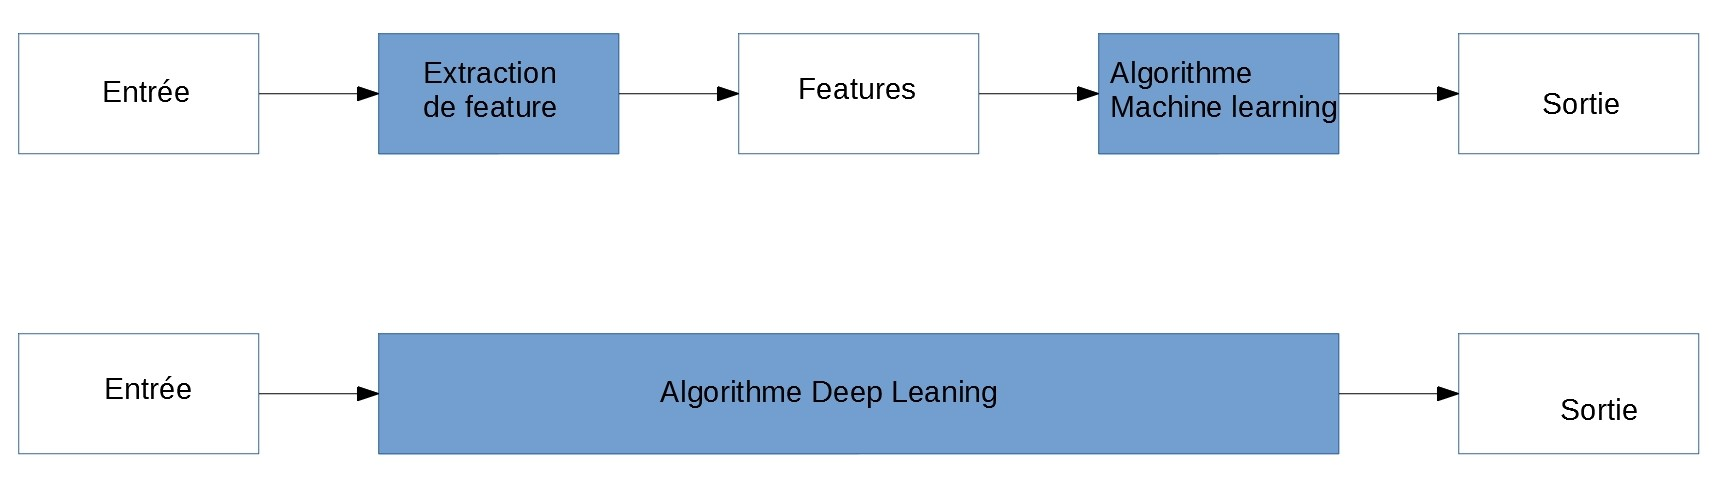
\includegraphics[width=1\textwidth]{Images/MLvsDL}
    \caption{Différences entre Shallow Learning et Deep Learning}
	\label{fig:DiffMLDL}
\end{figure}

Le Deep Learning contrairement au Machine Learning n'a pas besoin de selectionner
ou extraire manuellement les features, le modèle apprend par lui même à reconnaître
des features, les réseaux de neurones utilisés pour le Deep Learning
ont plus d'une couche caché de neurones d'où le nom "deep": \newline

\begin{figure}[H]
    \centering
    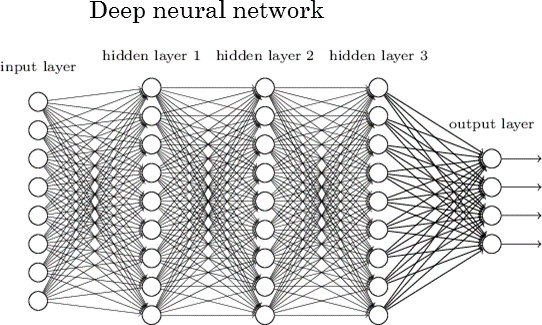
\includegraphics[width=0.7\textwidth]{Images/deepnn}
    \caption{Réseaux de neurones à 3 couches cachées}
	\label{fig:deepneuralnetwork}
\end{figure}

Ce qui fait la puissance du Deep Learning est sa capacité à avoir des représentations
intermédiaires d'un niveau d'abstraction faible à un niveau d'abstraction élevé:

\begin{figure}[H]
    \centering
    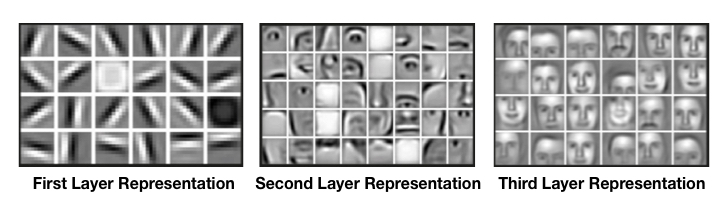
\includegraphics[width=1\textwidth]{Images/layeredrepresentation}
    \caption{Répresentations intermediaires - Andrew Ng}
	\label{fig:deepnnrepresentation}
\end{figure}

Ces représentations permettent de ne pas avoir à définir manuellement les features.
Dans l'exemple ci-dessus, l'algorithme extrait des features bas niveau dans la
première représentation, puis les assemble pour former des parties des
visages. Progressivement, l'IA obtient des représentations de features de plus en plus
haut niveau qui finissent par former des visages entiers. \newline

\chapter{Applications de l'Intelligence Artificelle}
Depuis ces dernières années, le Machine Learning est en essort à l'échelle mondiale.
Une grande majorité des entreprises de nos jours cherchent à implémenter l'utilisation de l'IA
afin de rester compétitifs sur le marché. \newline

En effet le Machine Learning, est un concept prometteur
et polyvalent sur la façon dont il peut se mettre en application.
Nous nous intéresserons ici à deux domaines proposant deux perspectives différentes
sur les apports ainsi que l'implémentation fonctionnelle de cette technologie.

\section{Le secteur de la Finance}
\subsection{Besoins et utilisations}
Jusqu'à il y a quelques années, la finance recrutait un nombre
important de personnes afin de répondre aux objectifs quotidien
que s'imposent les entreprises et institutions :\newline

\begin{itemize}

    \item Une sécurisation forte et maintenue dans le temps : \newline
    Le milieu bancaire est certainement là où ce besoin se fait les plus ressentir.
    Des équipes entières d'inspecteurs sont formées afin d'analyser
    l'activité des comptes de chaque client
    afin de détecter des activités frauduleuses ou au moins suspectes. \newline
    Les données qui transitent entre ces établissements sont également
    enviées par bon nombre de personnes mal intentionnées,
    elles vont chercher tous les moyens possibles d'accéder à ces données. Ainsi,
    des moyens conséquents sont mis sur la maintenance, la recherche et l'évolution
    des techniques de sécurisation des données et des réseaux informatiques. \newline

    \item Une création de valeur stable et croissant : \newline
    Toute organisation dépendant de la valeur générée cherche cela. \newline

    \item Une optimisation des coûts opérationnels : \newline
    Les processus mis en place doivent avoir parmis leurs objectifs de
    rester simple et optimisés, que ce soit au niveau des coûts
    ou au niveau du temps passé. \newline

\end{itemize}

\subsection{Avantages de l'IA par rapport à l'Homme}


\section{le secteur de la Médicine}
\subsection{Besoins et utilisations}
\subsection{Avantages de l'IA par rapport à l'Homme}

